% CREATED BY DAVID FRISK, 2016
\chapter{Background}
\textit{In this chapter a general glance on Artificial Intelligence, and its sub-categories, is given.}\\\\

\epigraph{ \textit{Can a machine think?}}{--- \textup{Alan Turing}, Computing Machinery and Intelligence}

\section{Overview}
In the past decade many companies have started to advertise the use of AI, even if they are using a subfield of the AI, in their products and software applications. Nevertheless, the exponential growth of the last decade,
the AI is not youth.\\ it takes one of its roots from a theoretical paper of \textit{Alan Turing} published by journal \textit{Mind} in the 1950 \cite{paper:36}.\\

The general definition of Artificial Intelligence (AI) is intelligence demonstrated by machines, any device that perceives its environment and takes actions that maximize its chance of successfully achieving its goals.\\ Colloquially, the term "artificial intelligence" is often used to describe machines that mimic "cognitive" functions that humans associate with the human mind, such as "learning" and "problem solving" \cite{book:1}.\\
Given the definition, it is evident that the AI is to vast to be studied and simulated. Thus, it has been divided into subfields, characterized by different traits, such as Knowledge Representation, Planning, Learning, Natural Language processing, Perception, Motion and manipulation, Social intelligence, General Intelligence.\\\\

Artificial Intelligence, like electricity or the fuel engine, is a general purpose technology. There is no consensus on which tasks AI tends to excel and how to characterize them.

\begin{figure}
\centering
\captionsetup{justification=centering}
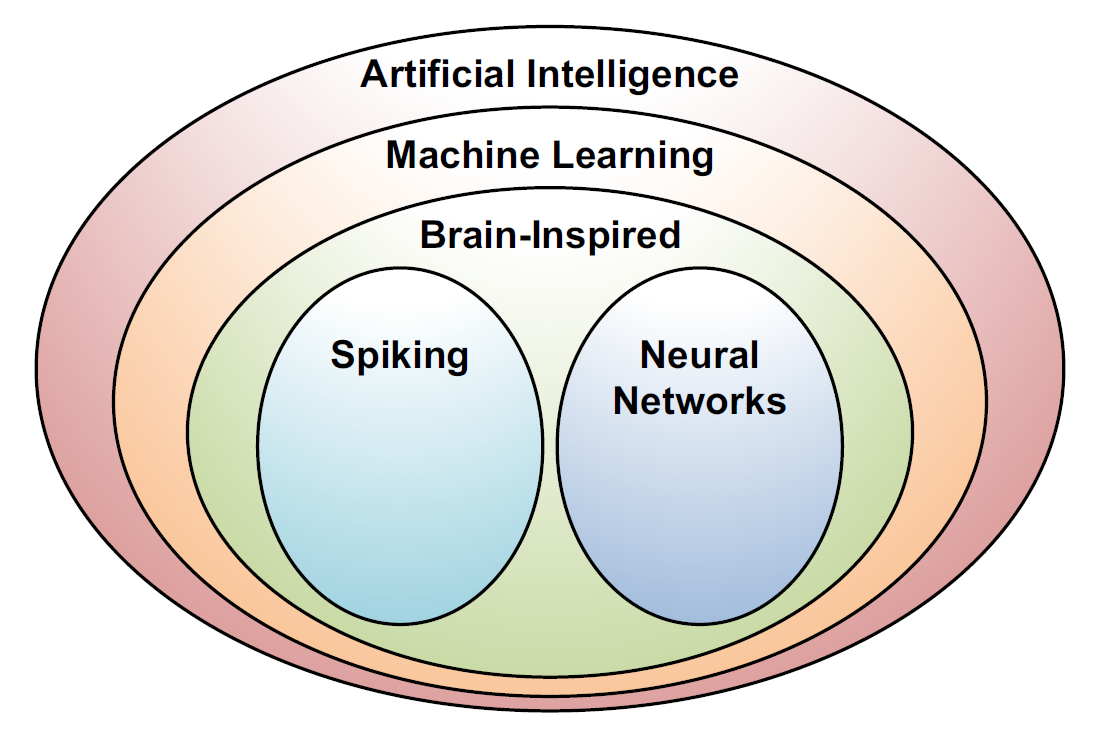
\includegraphics[scale=0.5]{./figure/ai_division.PNG}
\caption{Classification of AI with emphasis on Machine Learning and its subclassification}
\label{fig:aidiv}
\end{figure}

\section{Machine Learning}
A particular interesting subcategory of AI in Computer Science is the Machine Learning. It is the study of algorithms used to perform a specific task without explicit programming the machine, relying on patterns and inference, in order to make decisions. This approach is used where it is tricky, or unfeasible, to develop a conventional algorithm for solving the task.\\

A peculiarity of Machine Learning model is that it is composed of two processes, training and inference.
\todo[inline] {describe two processes}

As it can be seen in Figure \ref{fig:aidiv} Machine Learning is also divided in subcategories.
\subsection{Brain Inspired}
It is based on algorithms which take its basic functionalities from our understanding of how the brain operates.

\subsubsection{Neural Networks}

\subsubsection{Spiking}

\section{Applications}
In principle the AI can be applied to any intellectual tasks. Focusing on Machine Learning applications, they can spread through a variety of different domains:
\begin{itemize}
\item Healthcare, mainly used for classification purposes.
\item Automotive, used in self-driving cars.
\item Finance and economics, to detect charges or claims outside the norm, flagging these for human investigation. In banks system for organizing operations, maintaing book-keeping, investing in stocks and managing properties.
\item Cybersecurity, automatically sort the data in networks into high risk and low-risk information.
\item Government, for paired with facial recognition systems may be used for mass surveillance.
\item Video games, it is routinely used to generate dynamic purposeful behavior in non-player characters.
\item Military, enhancing C2, Communications, Sensors, Integration and Interoperability.
\item Hospitality, to reduce staff load and increase efficiency.
\item Advertising, it is used to predict the behavior of customers from their digital footprint in order to target them with personalized promotions.
\item Art, it has inspired numerous creative applications including its usage to produce visual art.
\end{itemize}
However, all the Machine Learning applications are characterized by the need of a huge amount of data set for the training process.